\section{System architecture}
\label{sec:arch}

\subsection{Runtime overview}
\label{sec:arch-overview}

Figure~\ref{fig:arch} shows the platform. Three cooperating sides share one
runtime process. The \emph{agent collaboration runtime} hosts workspaces,
channels, agent teams (a lead that decomposes goals and supervises workers,
plus workers that execute tasks), per-channel event buses with sequenced
delivery, shared process memory, and mailboxes. Agents are executed by
pluggable \emph{harness adapters}. Fourteen adapters cover in-process
engines, RPC subprocess engines, ACP-style engines, served engines, and
headless CLI engines, so that the same governed operation surface is
exposed regardless of which LLM backend a team runs. The \emph{governance
block} holds the operation catalog and the per-call checks described in
this section. The \emph{industrial side} comprises the data-acquisition
gateway with per-node edge runtimes, the write-control gateway, protocol
drivers for five field protocols plus a serial plugin and a MES REST
integration, and the time-series store. The store is embedded SQLite by
default, or TimescaleDB with daily chunks and compressed columnstore when
provisioned.

\begin{figure}[!t]
\centering
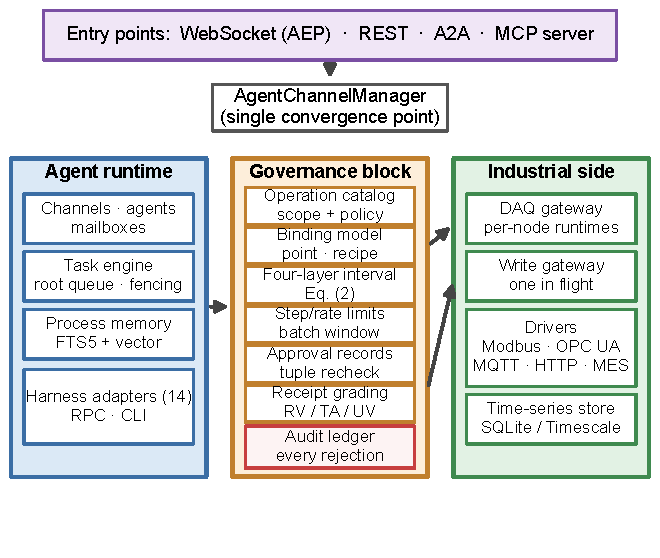
\includegraphics[width=0.98\columnwidth]{figures/fig1-architecture.pdf}
\caption{Platform architecture. Agent teams run inside the collaboration
runtime through pluggable harness adapters; all plant-facing operations
cross the governance block, which evaluates binding scope, the four-layer
admission interval, approval records, and receipt grading, and writes every
decision to the audit ledger. The industrial side separates acquisition
from write control and persists telemetry in an embedded or provisioned
time-series store.}
\label{fig:arch}
\end{figure}

Four entry points (WebSocket, REST, A2A, and an in-process MCP server
\cite{mcp2024,silva2025mcpmanufacturing}) converge on the same
AgentChannelManager, so that an operation is governed identically no matter
where it originates. This convergence is deliberate: it prevents the
common failure mode in which an interactive path is governed but a
programmatic path is not.

\subsection{Configuration-driven binding model}
\label{sec:arch-binding}

\textbf{Production context as configuration.} The platform's configuration
model describes the plant as \emph{scenes}: a scene declares lines; a line
declares products; a product declares recipes; a recipe declares
parameters with engineering windows. A line run instantiates a
line--product--recipe tuple and opens a batch. Nodes are typed as
acquisition nodes (readable plant points) or write-control nodes
(writable plant points). Each carries protocol driver configuration, a
structural safe range, and semantic metadata (meaning, unit, engineering
interpretation). All of this is data (one declarative source with
declared defaults), not code. A running configuration therefore answers,
for any moment, \emph{what is being produced, under which recipe, with
which windows, on which nodes}.

\textbf{Agent authority.} Agent authority is bound to this structure
through three binding tracks. A \emph{point binding} ties an agent to
specific write-control nodes; the set of values an agent may dispatch is
the intersection of the requested set with the bound set, so a binding
narrows rather than grants. A \emph{recipe binding} grants operations on a
single recipe; a \emph{line-recipe binding} grants operations across all
recipes of a line. Binding modes are \emph{manual} (every dispatch waits
for human approval) or \emph{auto}; switching a binding to auto requires an
explicit confirmation action, never a side effect of normal use.
Separately, users hold tri-state line permissions (none, view, operate);
the data plane filters by permission before any agent-level check, so an
agent bound to a node the user cannot operate still yields no data.

Direct node-write operations are refused by design: the tool family that
would bypass the governed path exists only as a single-source declaration
whose handlers reject unconditionally, keeping the write path non-bypassable
from the agent surface. Agent-facing tool descriptions are injected from
the same configuration (semantic cards derived from node metadata, line
condition, and associated devices). Thus, the agent's view of a node
carries its engineering meaning, and the model is not trusted to have
remembered it.

\textbf{Shared dispatch condition.} Every plant-facing operation request
$(a, c, u)$ (agent $a$, capability $c$, and unit of work $u$) is
admitted by a conjunction of predicates drawn from the governance block:
\begin{equation}
\mathcal{A}(a,c,u) \;=\; \bigwedge_{X \in \mathcal{C}(u)} X(a,c,u),
\qquad \mathcal{C}(u) \subseteq \{S, P, G, B\},
\label{eq:dispatch}
\end{equation}
where $S$ is scope (the agent holds the binding for $c$ on $u$), $P$ is the
channel policy under which $a$ runs, $G$ is any applicable grant, and $B$
is the operation-specific binding predicate. $\mathcal{C}(u)$ always
contains $S$ and $P$; $G$ and $B$ attach for the write-path operations
discussed next. Each predicate records its own verdict, which is what makes
the eventual audit layer-attributable rather than binary.

\subsection{The governed write path}
\label{sec:arch-write}

Figure~\ref{fig:writepath} traces a setpoint write through the path. The
stages realize R2--R6. Individually, these mechanisms have precedents in
industrial practice: engineered-range limit checks, post-write
verification, approval workflows with audit trails. What follows states
them precisely so that their \emph{composition} can be evaluated rather
than assumed: the composition adds separately attributable verdicts,
receipts graded by device-side evidence, and the absence of a bypass from
the agent surface.

\textbf{Walkthrough.} The running example of Section~\ref{sec:intro} is
admitted in five observable steps. (i)~R1: the binding query resolves the
node and the recipe; a missing binding rejects before any driver call.
(ii)~R2--R3: the four-layer interval intersects the node's hard range with
the active product and recipe windows; a value outside the intersection
returns the excluding layer, and the hard range is never administratively
relaxed. (iii)~R4: a manual binding creates an approval record carrying the
candidate value, the applicable limits, an expiry, and the
line--product--recipe--run tuple; dispatch rechecks the tuple and limits.
(iv)~R5: the driver executes; the platform reads the value back and grades
the receipt, reporting a transport acknowledgment as such. (v)~R6: every
prior verdict, including the rejection path, is appended to the ledger.
The example is deliberately ordinary: the design claim is that no step can
be skipped from the agent surface.

\begin{figure}[!t]
\centering
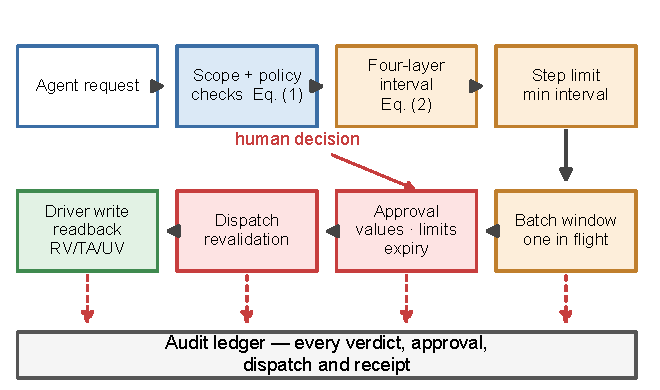
\includegraphics[width=0.98\columnwidth]{figures/fig2-writepath.pdf}
\caption{The governed write path. A machine-originated setpoint write
crosses scope and policy checks, the four-layer admission interval, rate
and step limits, a human approval record with tuple recheck, dispatch-time
revalidation, driver execution, readback verification, and receipt grading;
every stage's verdict, including rejections, lands in the audit
ledger. Rejection paths are drawn dashed.}
\label{fig:writepath}
\end{figure}

\textbf{Four-layer admission interval.} For a write-control node $n$ at
time $t$, the admissible value interval is
\begin{equation}
\mathcal{I}^{\mathrm{online}}_n(t) \;=\;
\mathcal{H}_n \;\cap\; \mathcal{L}^{\mathrm{base}}_n
\;\cap\; \mathcal{L}^{\mathrm{prod}}_n(t)
\;\cap\; \mathcal{L}^{\mathrm{rec}}_n(t),
\label{eq:interval}
\end{equation}
the intersection of the node's hard engineering range $\mathcal{H}_n$
(structural, not administratively relaxable), the parameter baseline
limits, the limits of the product currently in production, and the
parameter window of the recipe currently in production. A value outside
the intersection is rejected, and the response identifies the excluding
layer. The layers are evaluated in this fixed order, so two writes
rejected by different layers produce observably different records (M2).

\textbf{Rate and step limits.} Online writes additionally pass a per-node
step limit (a node without a configured step limit rejects online writes
rather than inheriting a default), a minimum interval between successive
writes, and a cooldown after a failed write. These limits apply
uniformly across protocol drivers; a driver cannot opt out.

\textbf{Batch-window interlock.} When a line run is active, writes are
admitted only within the run's batch window, and only one proposal per
actuator may be in flight. A second proposal, even from a different
agent team, waits or is refused, and a human arbitrates conflicting
intents. This interlock is deliberately \emph{soft}: it is the layer the
evaluation ablates (Section~\ref{sec:eval-ablation}), which requires that
the platform can run with it disabled. Disabling it does not disable the
hard range: R3 is preserved by construction, and the ablation confirms it
empirically.

\textbf{Bound approval.} For bindings in manual mode, the write dispatch
suspends and an approval record is created. The record binds the requesting
actor, the proposed operation and candidate values, the applicable limits
at proposal time, an expiry (a configurable setting; default 180\,s, with
the decision defaulting to rejection on timeout), and the active
line--product--recipe--run tuple. The
human approves or rejects in a dedicated surface; the platform never
writes on the agent's behalf while approval is pending. Recipe-level
operations (promoting a full parameter set) carry a separate, stricter
approval gate with the approver's stated basis returned verbatim into the
record.

\textbf{Dispatch-time revalidation.} Approval is not a capability token.
At dispatch, the path revalidates the approver's authority and compares
the current line--product--recipe--run tuple, the applicable limits, and
the approval expiry against the record; any mismatch fails the dispatch
closed (M3). The same revalidation runs again at the execution point after
queueing, bounding the window between decision and device contact.

\textbf{Receipt grading.} After driver execution the platform grades the
outcome. Where the driver provides a read channel, the written value is
read back (a mismatch triggers up to three re-reads at 2\,s intervals to
absorb actuator settling). The receipt is then \emph{readback-verified}.
A protocol-level success status alone does not qualify: an OPC UA Write
service result, for instance, reports server-side application rather than
physical effect, which is precisely why the top grade requires a readback.
Where the integration path provides only an acknowledgment, the receipt is
\emph{transport-acknowledged}; the platform states explicitly that this
class does not establish that the device applied the value. Where neither
exists, the receipt is \emph{unverified}. Downstream consumers, including
agents, receive the grade with the result text, so a report that cites a
write also cites its evidence class (M4).

\textbf{Total ledger.} Every stage verdict is appended to the audit ledger:
admission decisions with the deciding layer and excluding interval, approval
creations, approvals and rejections with actor and basis, revalidation
failures, dispatch attempts, and receipts with grades. Rejections are
first-class records, not silent drops. The ledger is the substrate for
Section~\ref{sec:eval-ablation}'s mechanism attribution: an ablation arm
can be shown to have executed window-breaching writes \emph{because the
ledger says so}, even when the platform had no power to stop them.

\subsection{Acquisition, context, and agent runtime}
\label{sec:arch-daq}

On the read side, each acquisition node runs an edge runtime with an
ingest cadence and an independent publication cadence (capped for
interface backpressure). A gateway sweeps drivers on a fixed 250\,ms
cycle with in-flight mutual exclusion, drops out-of-order frames, and
rejects future timestamps rather than persisting them. Persistence is
gated on an \emph{active batch}: telemetry outside an active line run is
served live but not written to history, which keeps the analytical store
aligned with production context. Recipe-window breaches observed on
acquired values raise alarm edges from the same runtime that persists
samples, so monitoring and history cannot diverge.

Agents perceive the plant through a bounded tool surface: history queries
with statistics, current-value reads, node discovery scoped by bindings,
and the governed write operations of
Section~\ref{sec:arch-write}. The task runtime is a seven-state machine
(SUBMITTED, ASSIGNED, WORKING, WAITING, COMPLETED, FAILED, CANCELED) with a
root-queue and lease fencing; leads re-dispatch failed tasks under budget.
A regulation workflow template (observe, understand, hypothesize,
propose, await decision, verify, review) is injected into supervisory
prompts together with the semantic cards of Section~\ref{sec:arch-binding}.
Its constraint set (goals must land inside the safe range intersected
with the recipe window; single steps bounded to a small fraction of the
range) mirrors the path's own limits. The agent is thus asked to do
nothing the path would refuse.

\subsection{Model-driven optimization tier}
\label{sec:arch-opt}

Agents do not have to propose setpoints from raw reasoning alone. An
optional model tier (automated machine learning over acquired process
data) produces process models that agents can solve against. The tier is
gated so that model quality claims are platform-recomputed rather than
self-reported. Training jobs produce candidates. Promotion to
reference-grade status requires passing a gate set that includes
single-step and rolling prediction error bounds, a generalization gap
bound, and minimum data-volume requirements, evaluated by the platform on
held-out data. Uncertainty calibration (conformal bounds over a residual
ensemble on top of a physics-prior core with clamped residual scale) and
out-of-distribution rejection are part of the model contract. A trial
service simulates candidate setpoint moves against a gated model before
any plant contact and marks trial outcomes as simulation evidence;
candidates that pass a twin gate may then be bound to a channel, and only
bound models enter the optimizer surface.

The optimizer itself compiles a problem intermediate representation with a
content hash (model artifacts, MV domains taken strictly from node specs
including step limits, CV targets) and solves it with OSQP over a dense
sensitivity expansion, with movement and hard-domain constraints. A
steady-state variant uses SLSQP. Two independent services, the solver
and the digital twin \cite{jones2020characterising}, recompute the same
objective from the same frozen
inputs and must agree to within $10^{-6}$ relative tolerance before a
result is surfaced; model artifact hashes are cross-checked, so the
dual-check cannot silently span different model revisions. Dispatched
recommendations re-enter the governed write path of
Section~\ref{sec:arch-write}: the optimizer has no private path to the
plant. Recipe trials run at a bounded cadence with a declared hypothesis;
an outcome that meets the hypothesis promotes the recipe version (with a
second human approval). One that does not rolls back through a
unified rollback service that restores the previous version and, where the
driver supports it, rewrites the affected plant values as a batch. Judge
and executor are separate services, so the component that decides a trial
failure is not the component that performs the rollback.
